\documentclass[10pt,a4paper]{article}
\usepackage{tabu}
\usepackage{amsmath}
\usepackage{amsfonts}
\usepackage{amssymb}
\usepackage{makeidx}
\usepackage{graphicx}
\usepackage[backend=biber]{biblatex}
\usepackage{textcomp}
\DeclareMathSizes{12}{30}{16}{12}
\usepackage[margin= 1in]{geometry}
\graphicspath{ {Images/} }
\usepackage{listings}
\usepackage{float}
\addbibresource{bibliography.bib}
\usepackage{color}

\author{James Walker-Wilson}
\title{Sound Level Meter}
\makeindex
\definecolor{codegreen}{rgb}{0,0.6,0}
\definecolor{codegray}{rgb}{0.5,0.5,0.5}
\definecolor{codepurple}{rgb}{0.58,0,0.82}
\definecolor{backcolour}{rgb}{0.95,0.95,0.92}
 
\lstdefinestyle{mystyle}{
    backgroundcolor=\color{backcolour},   
    commentstyle=\color{codegreen},
    keywordstyle=\color{blue},
    numberstyle=\tiny\color{codegray},
    stringstyle=\color{black},
    basicstyle=\footnotesize,
    breakatwhitespace=false,         
    breaklines=true,                 
    %captionpos=b,                    
    keepspaces=true,                 
    numbers=left,                    
    numbersep=5pt,                  
    showspaces=false,                
    showstringspaces=false,
    showtabs=false,                  
    tabsize=2
}
 
\lstset{style=mystyle}
\begin{document}
\maketitle
\newpage

\begin{abstract}

\end{abstract}

\section{Introduction}
This report outlines the design and construction of a sound level meter. The device measures the sound level of the environment. This is the filtered through several filter stages and the sound level is displayed on an LED bar graph. The sound signal is filtered to select a band of frequencies and then low pass filtered to produce a DC voltage level proportional to the sound level.  

\subsection{Aims}
\begin{itemize}
  \item To understand the design of a common emitter amplifier for the first stage.
  \item To understand the design of an LC band pass filter.
  \item To understand the construction and operation of a signal rectifier.
  \item To understand the construction of a low pass filter.
  \item To understand how to program a PIC Micro controller.
  \item To understand the construction and testing of the circuit.  

  \end{itemize}

\subsection{Objectives}
\begin{itemize}
  \item To determine the $\beta$ of the transistor by experimentation
  \item To design a common emitter amplifier for the first stage of the circuit with appropriate gain
  \item To design an LC band pass filter and calculate the number of turns of wire to create the required inductance.
  \item To construct a rectifier to rectify the signal
  \item To construct a low pass filter to convert the signal to a dc voltage level.
  \item To create a program to change the number of LED's that are on depending on the sound level and program the Micro controller with the code.
  \item To test the completed stages and whole circuit to make sure it operates as intended.  

  \end{itemize}

\section{Method}

\subsection{Design}
\subsubsection{Determining $\beta$}
To determine $\beta$ the circuit shown in figure \ref{Beta}. $R_C$ was set to $3.9K\Omega$. $R_B$ was then chosen to make $V_{CE}\approx 7.5V$. The base current was calculated by measuring the voltage across $R_B$ and using Ohms law, the same was done for the collector current. To work out $\beta$ the formula
\begin{center}
\Huge
$\beta = \frac{I_C}{I_B}$
\end{center}
was used. This gave a value of $\beta = 337$.

\begin{figure}[!h]
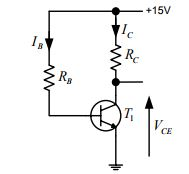
\includegraphics[scale=0.7]{beta}
\caption{Circuit used to determine $\beta$}
\label{Beta}
\end{figure}
\newpage
\subsubsection{Common Emitter Amplifier}
The first stage of the circuit is a common emitter amplifier to amplify the signal from the microphone to be processed by later stages. The transistor $\beta$ was found to be $\beta = 337$. First the current $I_C$ was calculated using the equation with $V_C = 7.5V$ and $ R_3 = 3.9K\Omega$ \newline
\begin{center}
\Huge
$I_c = \frac{15-V_c}{R_3}$
\end{center}
This equation gives an $I_c$ value of $ I_c = 1.92mA$. $R_4$ is then calculated with the equation
\begin{center}
\Huge
$R_4 = \frac{1.5}{I_E}$
\end{center}
with $I_e \approx I_c$ this makes $R_4= 781 \Omega$. To calculate the biasing resistors it is set that the current through the biasing resistors is $10\times I_B$. The equation 
\begin{center}
\Huge
$R_2 = \frac{V_{BE} + V_E}{10\times I_B}$
\end{center}
This gives an $R_2 \approx 40K\Omega$
$R_1$ can then be calculated with the equation.
\begin{center}
\Huge
$R_1 = \frac{V_{CC}-V_B}{10\times I_B}$
\end{center} 
This gives $R_1 \approx 27K\Omega$
\begin{figure}
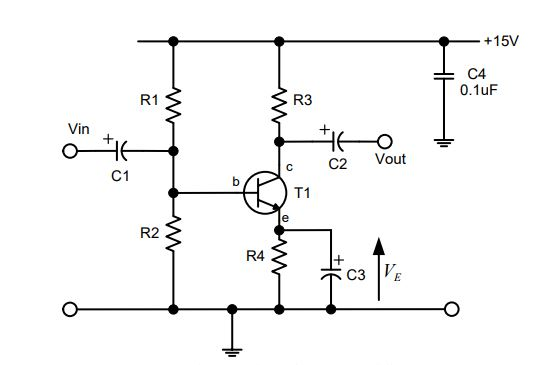
\includegraphics[scale=1]{CircuitDiagram}
\caption{Common emitter amplifier circuit diagram}
\end{figure}

\subsubsection{Bandpass Filter}
The band pass filter uses a resonant LC circuit to set the filter characteristics. The resonant frequency of an LC circuit is given as 

\begin{center}
\Huge

$f = \frac{1}{2\pi\sqrt{LC}}$

\end{center}

The capacitor that forms the resonant circuit is $C5 = 1\mu F$
to calculate the value for $L$ the equation is rearranged to 
\begin{center}
\Huge

$L = \frac{1}{(2\pi f)^2 C}$

\end{center}
This gives $L = 11.3mH$. To calculate the number of turns on the inductor the equation

\begin{center}
\Huge

$N= \sqrt{\frac{Ll}{\mu \times a}}$
\normalsize
\newline
$L=$ Inductance,$l=$ length of magnetic circuit,$\mu=$ permeability and $a=$ cross sectional area. 

\end{center}


is used. This gives $N=61$ Turns.

\begin{figure}[!h]
\label{BPF}
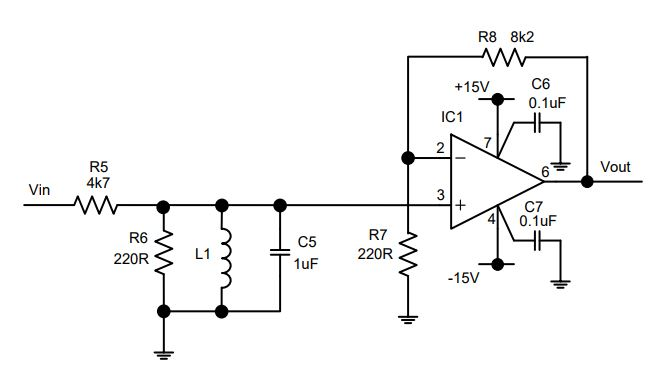
\includegraphics[width= \textwidth]{Bandpass}
\caption{Band pass filter circuit diagram}

\end{figure}
\subsubsection{Code}
The code was made to light all the LED's when maximum sound level was achieved. This was done with a logarithmic scale to allow high sensitivity at low sound levels but allow a large range of sound levels to be measured without clipping at high end values.

\begin{tabu} to 0.8\textwidth { | X[c] | X[c] |}
 \hline
 Number of bars lit & Voltage level(mV)\\
 \hline
 0 & 0\\
 \hline
 1 & 1.8\\
 \hline
 2 & 3.28\\
 \hline
 3 & 5.94\\
 \hline
 4 & 10.76\\
 \hline
 5 & 19.49\\
 \hline
 6 & 35.3\\
 \hline
 7 & 63.95\\
 \hline
 8 & 115.8\\
 \hline
 9 & 209\\
 \hline
 10 &380\\
 \hline

\end{tabu}
\newline
These values were then used to create the code 
\begin{lstlisting}[language= C]
//Newcastle University - EEE - Stage 1 - Sound Level Meter
//16F819 PIC software to drive a 10-LED bargraph display from a dc level on ADC input 0 (AN0).
//Port A and B used to drive LEDs.
//Pin Configuration:
//Pin Configuration:
//1-RA2 (LED4) 18-NC
//2-RA3 (LED3) 17-AN0 (DC Sound Level input)
//3-NC 16-RA7 (LED1)
//4-MCLR 15-RA6 (LED2)
//5-VSS 14-VDD
//6-RB0 (LED10) 13-RB7 (PGD)
//7-RB1 (LED9) 12-RB6 (PGC)
//8-RB2 (LED8) 11-RB5 (LED5)
//9-RB3 (LED7) 10-RB4 (LED6)
#include <xc.h> //header file for device
#include <stdint.h> //header file for standard types e.g uint8_t
//fuse settings to configure device
//i.e. NOWDT - No Watchdog Timer, INTOSCIO - Internal clock used, pins available for I/O
#pragma config MCLRE = ON, CP = OFF, CPD = OFF, BOREN = OFF, WDTE = OFF
#pragma config PWRTE = OFF, FOSC = INTOSCIO, LVP = OFF, DEBUG = ON
void main()
{
 //*** INSERT ANY VARIABLE DECLARATIONS HERE ***
 //uint8_t = 8-bit unsigned number
 //unint16_t = 16-bit unsigned number
 uint16_t value;
 //*** The following code initializes the PIC ***
 OSCCONbits.IRCF = 0b111; //use internal 8MHz clock (FOSC=8MHz)
 TRISB = 0b00000000; //Port B all outputs
 TRISA = 0b00110011; //Port A B6/B7/B3/B2 outputs
 ADCON1bits.ADFM = 1; //A/D Result Format Right Justified
 ADCON1bits.ADCS2 = 1; //A/D clock Source divided by 2
 ADCON1bits.PCFG = 0b1110; //Enable AN0 input for sound level ADC
13
 ADCON0bits.ADCS = 0b01; //set ADC clock, should be between 1.6us and 6.4us (1/8MHz x 16 = 2us)
 ADCON0bits.CHS = 0b000; //select AN0 for input
 ADCON0bits.ADON = 1; //A/D Converter is operating
 do
 {
 //The code below will read the digital value from the 10-bit analogue to digital converter.
 //The range of the return value will be between 0 and 1023. Where 0V = 0 and 5V = 1023.
 //For example 2.5V on the ADC will return 511 to the variable value below.
 ADCON0bits.GO_nDONE = 1; //start A/D conversion
 while(ADCON0bits.GO_nDONE == 1); //wait for A/D conversion to complete
 value = ADRESH; //read MSB of ADC result
 value = value << 8; //shift left 8 bits
 value = value + ADRESL; //read LSB of ADC result. value now contains a 10-bit ADC number
 //*** INSERT YOUR PROGRAM CODE HERE TO ILLUMINATE THE LEDs***
 //The basic requirement of your code is:-
 //(i) To use the variable value to determine which LED bars should be switched on.
 //(ii) To write the appropriate code to the output pins RB0-RB5 and RA2,RA3,RA6,RA7.
 //The PIC PORTA and PORTB registers should be used to output a value to the Port pins
 //PORTA=0b00001111; will output a binary number to port A. Bits 7,6,5,4=0 and Bits 3,2,1,0=1.
 //Alternatively PORTA=15; for decimal equivalent.
 //The parameter may also be a variable instead of a constant e.g. PORTA=value;
 
if(value = 0){
PORTA=0b11111111
PORTB=0b11111111

}  
 
if(value > 0 && value <= 1.8){
PORTA=0b01111111
PORTB=0b11111111

} 

if(value > 1.8 && value <= 3.28){
PORTA=0b00111111
PORTB=0b11111111

} 

if(value > 3.28 && value <= 5.94){
PORTA=0b00110111
PORTB=0b11111111

} 

if(value > 5.94 && value <= 10.76){
PORTA=0b00110011
PORTB=0b11111111

} 

if(value > 10.76 && value <= 19.49){
PORTA=0b00110011
PORTB=0b11011111

} 

if(value > 19.49 && value <= 35.3){
PORTA=0b00110011
PORTB=0b11001111

} 

if(value > 35.3 && value <= 63.95){
PORTA=0b00110011
PORTB=0b11000111

}

if(value > 63.95 && value <= 115.8){
PORTA=0b00110011
PORTB=0b11000011

}

if(value > 115.8 && value <= 209){
PORTA=0b00110011
PORTB=0b11000001

}

if(value > 115.8 && value <= 209){
PORTA=0b00110011
PORTB=0b11000001

}




 
 
 
 
 
 
 } while (1);
}

\end{lstlisting}

\subsection{Construction}
\subsubsection{Common Emitter Amplifier}
After the common emitter amplifier was constructed on bread board using the resistor values determined in the design stage. This was to determine that the amplifier had been designed correctly. To test the design the voltage between the transistor collector and ground was measured and was found to be $V_C = 7.62V$. This is within the allowable limit of $6V$ to $9V$. The circuit was then constructed on the circuit board and the collector voltage was once again measured and found to be the same as before. The decoupling capacitors were then added to the circuit board. To test the amplifier a $20mV Pk-Pk$ sine wave at $1kHz$ was applied to the input and the output measured on an oscilloscope. This is shown in figure \ref{CEE}. Using an input of $23mV$ and an output of $4.3V$ leads to a gain of $G= 215$.

\begin{figure}[!h]



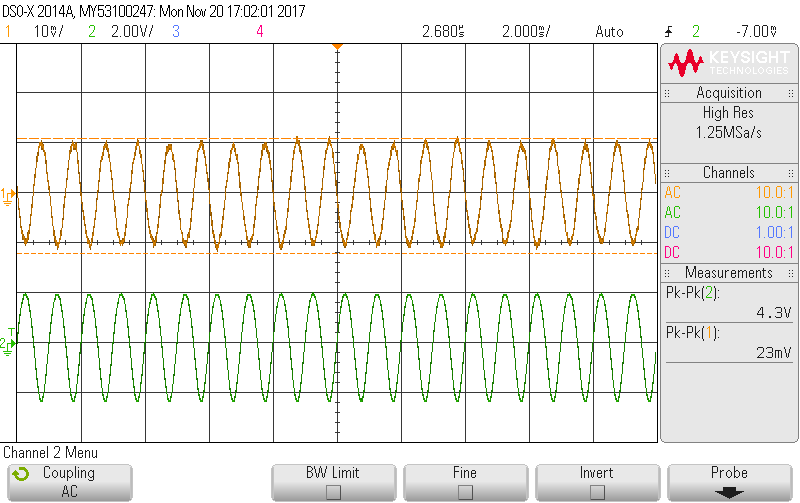
\includegraphics[width=\textwidth]{CEE}

\caption{Testing of the Common Emitter Amplifier}
\label{CEE}
\end{figure}
\subsubsection{Band Pass Filter}
To construct the band pass filter the Inductor must first be made. It was calculated that the required inductor would be made of 61 turns. This Inductor was created and its inductance was measured using an LCR meter. The desired inductance is $11.3mH$ however the inductance was measured as $11.9mH$, to reduce this turns were removed and the Inductor re measured until its inductance was equal to $11.3mH$. This was achieved with 56 turns. The circuit was then constructed on the circuit board according to the circuit diagram shown in Figure \ref{BPF}. Once completed the filter was characterised between $1Hz$ and $5kHz$ with a $2V Pk-Pk$ sine wave input shown in figure \ref{BandPassFilter}. 

\begin{figure}[!h]
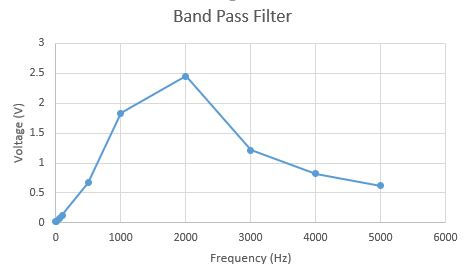
\includegraphics[width= \textwidth]{BPF}
\caption{Characterisation of Band Pass Filter}
\label{BandPassFilter}
\end{figure}
\subsubsection{Signal Rectifier}
The circuit shown in figure \ref{RecDia} was constructed on the circuit board and was then tested as shown in figure \ref{Rectifier} with a $1.5kHz$ $5V$ sine wave.





\begin{figure}[!h]
\includegraphics[scale= 0.75]{rectifierdia}
\caption{Rectifier Circuit Diagram}
\label{RecDia}
\end{figure}

\begin{figure}[!h]
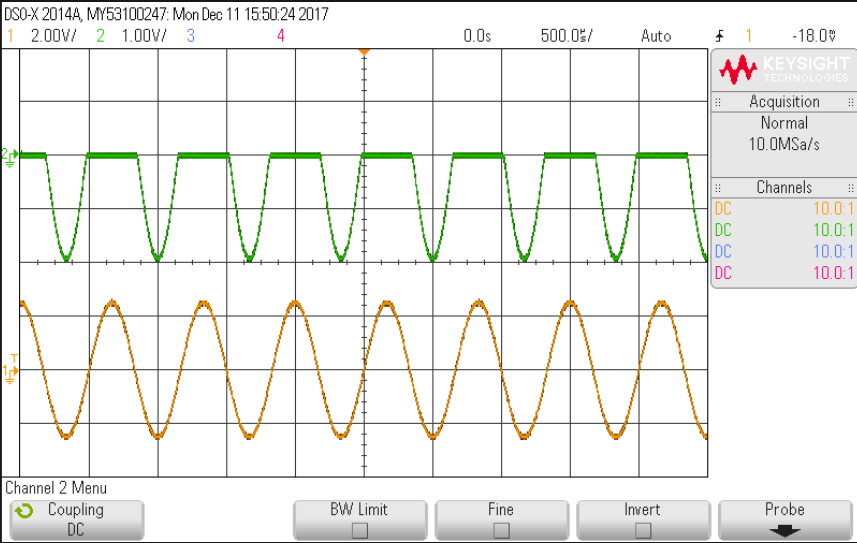
\includegraphics[scale= 0.5]{rectifier}
\caption{Rectifier analysis}
\label{Rectifier}
\end{figure}
\subsubsection{Low Pass Filter}
The Low Pass Filter was constructed on the circuit board according to the circuit diagram shown in figure \ref{LPF}. After the circuit was constructed it was tested by inputting a $1V Pk-Pk$ sine wave as shown in figure \ref{LPFscope}. The filter was then characterised between $1Hz$ and $1kHz$ with a $1V Pk-Pk$ input sine wave shown in figure \ref{LPFchar}. 

\begin{figure}
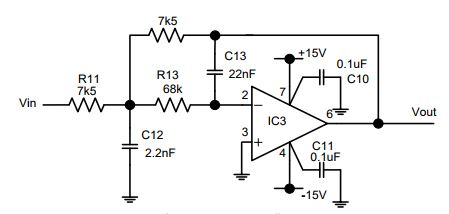
\includegraphics[width=\textwidth]{LPF}
\caption{Low Pass Filter Circuit Diagram}
\label{LPF}
\end{figure}

\begin{figure}[!h]
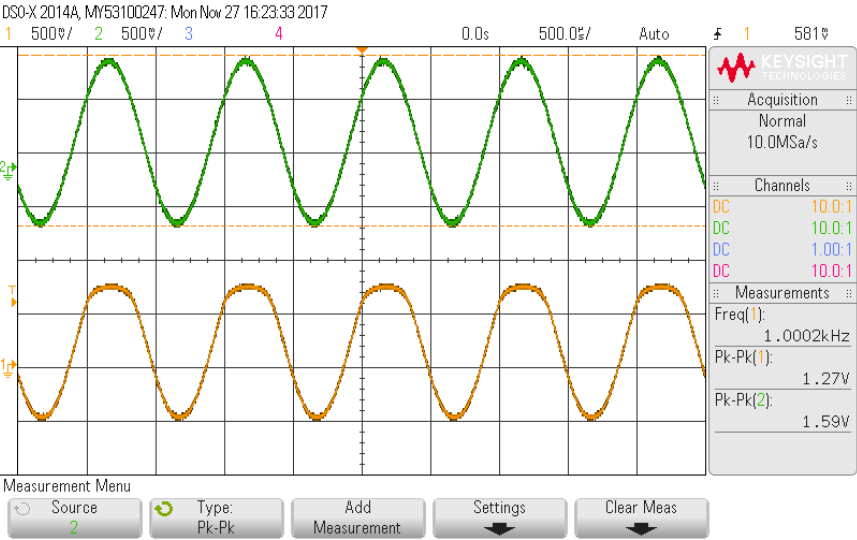
\includegraphics[width =\textwidth]{lpfilter}
\caption{Low Pass Filter input \& output}
\label{LPFscope}
\end{figure}

\begin{figure}[!h]
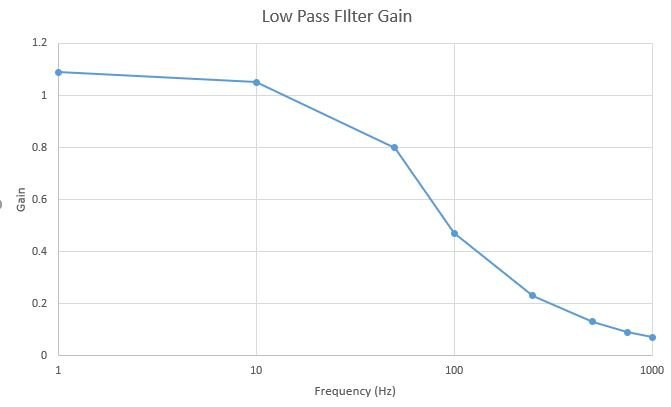
\includegraphics[width = \textwidth]{LPFchar}
\caption{Low Pass Filter Characterisation}
\label{LPFchar}
\end{figure}

\subsection{Analysis}

\section{Analysis}

\section{Conclusion}

\printbibliography

\end{document}
